\documentclass{beamer}
\usepackage[T1]{fontenc}
\usepackage[utf8]{inputenc}
\usepackage[british]{babel}
\usepackage{verbatim}

%verbeek: pag 52 cap 3

% see https://tex.stackexchange.com/questions/68080/beamer-bibliography-icon/68084#68084 for reference
\usepackage[style=authoryear,dashed=false,backend=biber]{biblatex}
\usepackage{hyperref}

\setbeamertemplate{bibliography item}{%
	\ifboolexpr{ test {\ifentrytype{book}} or test {\ifentrytype{mvbook}}
		or test {\ifentrytype{collection}} or test {\ifentrytype{mvcollection}}
		or test {\ifentrytype{reference}} or test {\ifentrytype{mvreference}} }
	{\setbeamertemplate{bibliography item}[book]}
	{\ifentrytype{online}
		{\setbeamertemplate{bibliography item}[online]}
		{\setbeamertemplate{bibliography item}[article]}}%
	\usebeamertemplate{bibliography item}}

\defbibenvironment{bibliography}
{\list{}
	{\settowidth{\labelwidth}{\usebeamertemplate{bibliography item}}%
		\setlength{\leftmargin}{\labelwidth}%
		\setlength{\labelsep}{\biblabelsep}%
		\addtolength{\leftmargin}{\labelsep}%
		\setlength{\itemsep}{\bibitemsep}%
		\setlength{\parsep}{\bibparsep}}}
{\endlist}
{\item}

% general data
\title{Smart Home Ambient Intelligence: \\voice assistants}
\subtitle{\vspace*{0.3cm}a new limit for our freedom?}
\author[Stefano Brandoli]{Stefano Brandoli}
\institute[PoliMi]{Politecnico di Milano\\Computer Ethics 2017/2018}
\date{December 12, 2017}

%theme and aspect
\setbeamertemplate{navigation symbols}{}
\addbibresource{bibliography.bib}
%\usetheme{metropolis}
\setbeamertemplate{section in toc}[circle]
\setbeamertemplate{subsection in toc}[ball unnumbered]
\setbeamerfont{subsection in toc}{size=\small}


\begin{document}

% frame
\begin{frame}
\maketitle
\end{frame}

% frame
\begin{frame}
\begin{center}\vspace*{-0.5cm}Smart Home Ambient Intelligence: voice assistants
	
a new limit for our freedom?
\end{center}
\frametitle{Presentation Outline}
\tableofcontents
\end{frame}

\section{Introduction}

% interleave
\begin{frame}
\begin{center}
	\usebeamerfont*{frametitle}
	\usebeamercolor[fg]{frametitle} Introduction
\end{center}
\end{frame}

\subsection{Technological Mediation}
% frame
\begin{frame}[fragile]
\frametitle{Technological Mediation}
\begin{quote}While fulfilling their function, technologies do much more: they \textbf{give shape to what we do} and how we experience the world. 
	And in doing so they \textbf{contribute actively} to the ways we live our lives (\cite{verbeek2011moralizing})
\end{quote}

\begin{itemize}
	\item Technologies are not \textbf{neutral intermediaries}
	%give shape to what we do and how we experience the world
	\item Technologies play an \textbf{actively mediating role} 
	%in the relationship between human beings and reality. No mute and passive objects
	\item Artifacts are \textbf{bearers of morality} (\cite{latour1992})
	%as they help people to make all kinds of moral decisions
	\item Morality is a matter of \textbf{human-technology associations}

\begin{comment}
%	not an exclusively human affair, since it requires intentions and freedom.
%	vs rigid separation of humans vs non humans in Latour words.
%	The only adequate way to understand it is in terms of its hybrid character.
%	it cannot be reduced to either an object or a subject but needs tounderstood in terms of their mutual relations. 
%moral action cannot be understood here
in terms of a radical separation of a human moral agent, on the one hand,
acting in a world of mute material objects on the other. 
\end{comment}

\end{itemize}

\begin{itemize}
	\item Two perspectives of mediation:
	\begin{itemize}
		\item Perception
		\item \textbf{Action}: I will focus on \textbf{human freedom}
		%Its central question is how human beings act in their world and shape their existence.
	\end{itemize}
\end{itemize}

\end{frame}

\subsection{Definitions}
% frame
\begin{frame}[allowframebreaks]
\frametitle{Definitions}	
	\begin{block}{Ambient Intelligence}
		\begin{quote}
			\textbf{Ambient Intelligence} is an approach that combines two major technologies: Ubiquitous Computing and Intelligent User Interfaces (IUIs)(\cite{brey2005freedom})
		\end{quote}
	\end{block}

	\begin{block}{Voice Assistant}
		\begin{quote}
			A \textbf{voice assistant} is a digital assistant that uses voice recognition, natural language processing and speech synthesis to provide aid to users through phones and voice recognition applications (\cite{whatis})
		\end{quote}
	\end{block}
	\framebreak
	\begin{block}{Freedom}
		   Two forms (Brey 2005, 2006):
		   
			\begin{itemize}
				\item Negative Freedom:
					\begin{itemize}
						\item act without obstruction or interference by others
						\item absence of limits and external constraints
					\end{itemize}
				example: artifact refusing to perform an action
				    \bigskip
					\item {\small \textbf{Positive Freedom (Human Autonomy)}: I will focus on this}
						\begin{itemize}
							\item mastery over your own life
							\item \textbf{think freely}, \textbf{make your own decisions} to act
							% and act based on those decisions
						\end{itemize}
			\end{itemize}
			
	\end{block}
\end{frame}

\section{Case Study: Google Home - Google Assistant Actions}

% interleave
\begin{frame}
\begin{center} 
	\usebeamerfont*{frametitle}
	\usebeamercolor[fg]{frametitle} Case Study: Google Home - Google Assistant Actions
\end{center}

\begin{figure}
	\centering
	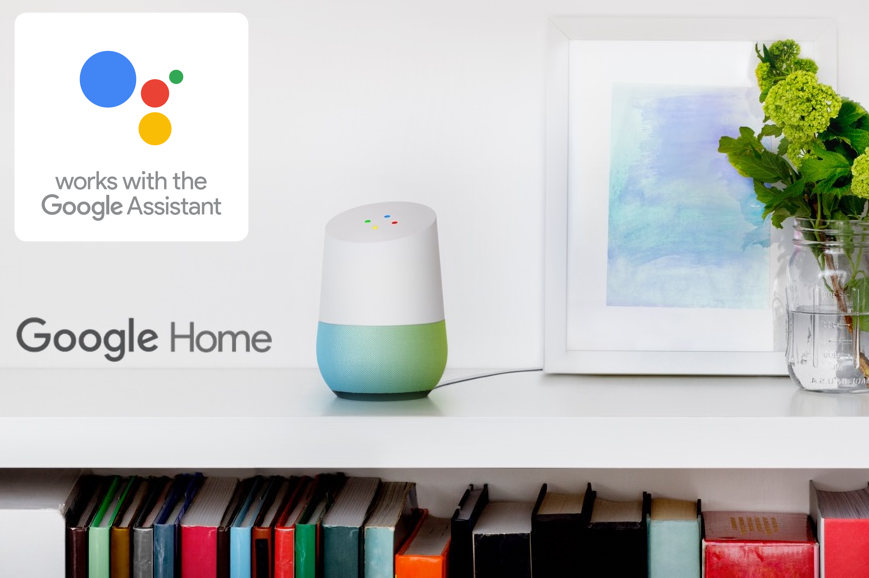
\includegraphics[width=1\linewidth]{images/Google-Home1}
	\label{fig:maxresdefault}
\end{figure}

\end{frame}

% frame
\begin{frame}
\frametitle{Google Assistant Actions}
\vspace{-0.5cm}
\begin{figure}
	\centering
	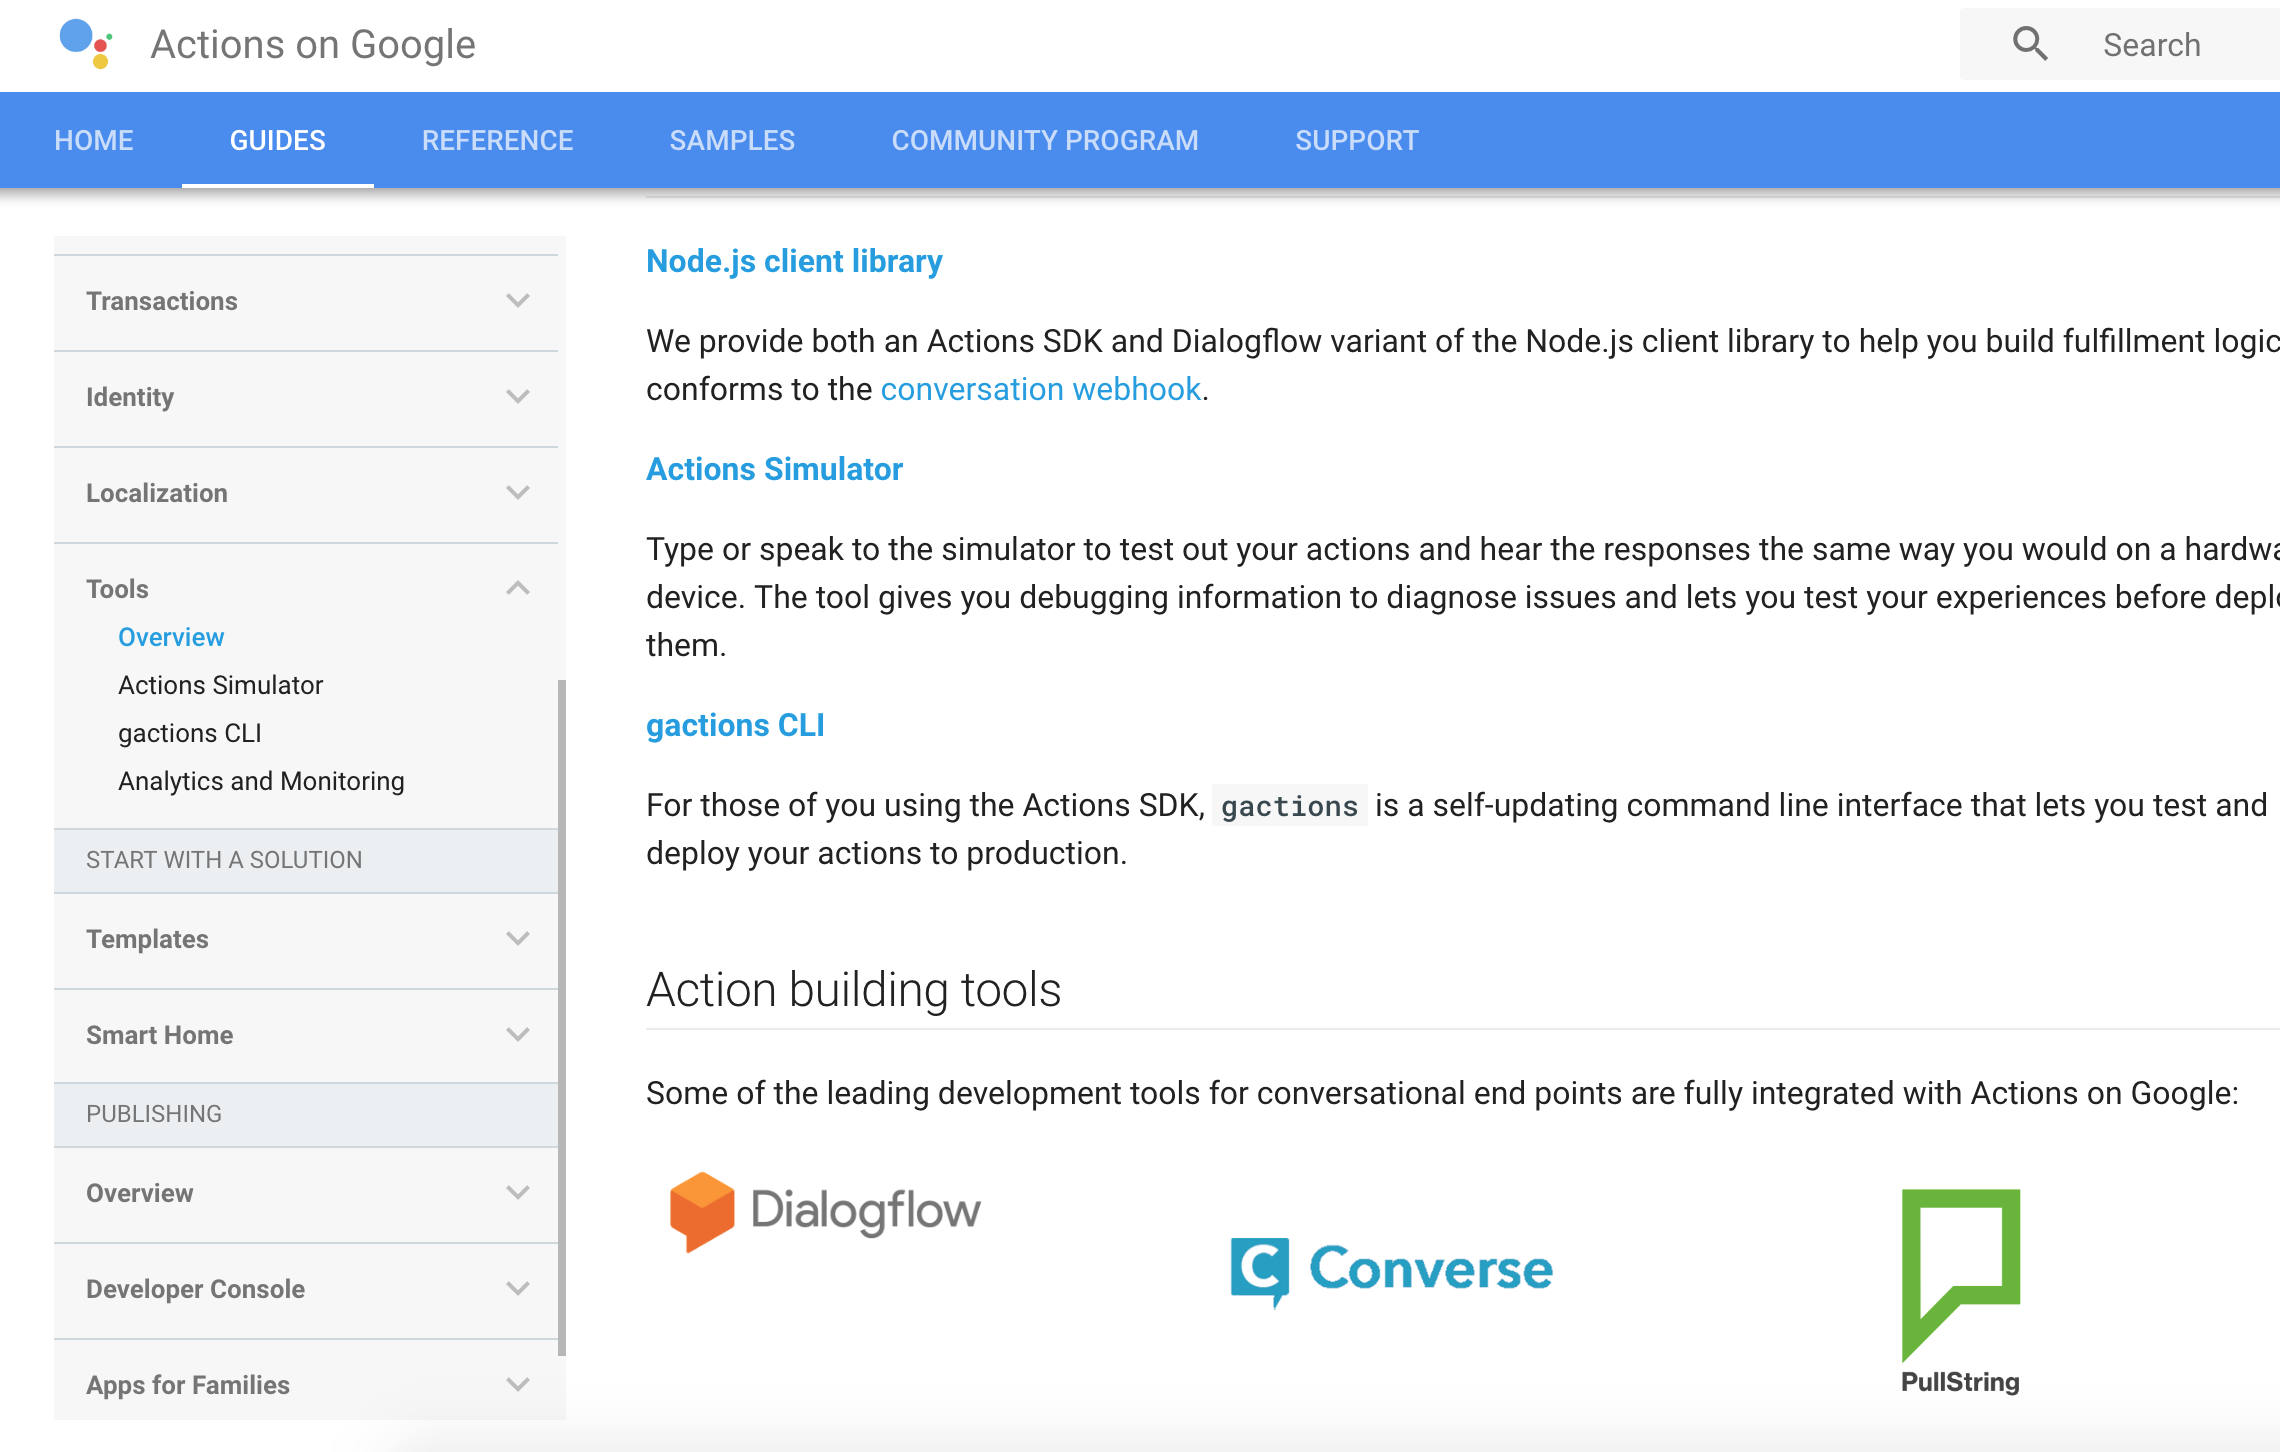
\includegraphics[width=0.85\linewidth]{images/documentation_preview}
	\label{fig:documentationpreview}
\end{figure}

{\small Starting from the \textbf{Actions on Google documentation} I will show:
\begin{enumerate}
	\item \textbf{Applied concepts} of Technological Mediation limiting our freedom
	\item \textbf{Ethical concerns} arising from loss of freedom
\end{enumerate}
}

\end{frame}

\subsection{Applied concepts of Technological Mediation limiting our freedom}
% interleave
\begin{frame}
\begin{center} 
	\usebeamerfont*{frametitle}
	\usebeamercolor[fg]{frametitle} Applied concepts of Technological Mediation\\limiting our freedom
\end{center}
\end{frame}

% frame
\begin{frame}
\frametitle{Script: make your own decisions}
% Developers design the whole conversational interaction. Pre-defined templates
% riferimento a quanto detto prima che giustifica il perchè del concetto

\vspace{-0.5cm}
\begin{block}{Script} 
	\begin{quote}
		A \textbf{script} is a prescription of  how to act when using the artifact (\cite{verbeek2011moralizing})
	\end{quote}
\end{block}

Interactions can be built in two ways (\cite{googleactions}):
\begin{itemize}
	\item \textbf{With templates}
			%most of the app's conversation and fulfillment is handled by the template
			\begin{itemize}
				{\small  \item \dots build apps \textbf{without writing a single line of code!}
				   %what about the future?
			 	 \item \dots build apps quickly \textbf{without worrying about designing conversations} \dots}
			 	 \item Google decides which interactions are good and what aren't
		\end{itemize}
		
		\medskip
	\item \textbf{Without templates}
		\begin{itemize}
			\item \textbf{Dialogflow}
			% built-in natural language understanding: don't have to define a fully exhaustive grammar
		    % Extract the data you need from user input
				\begin{itemize}
					\item machine learning
					\item natural language understanding
					\item extract parameters (data) from the user input
				\end{itemize}
			\item developers can decide the whole conversational interaction
			% define what users can say to your app 
		\end{itemize}
\end{itemize}

\end{frame}

\begin{frame}
\frametitle{Script: make your own decisions}
\begin{figure}
	\centering
	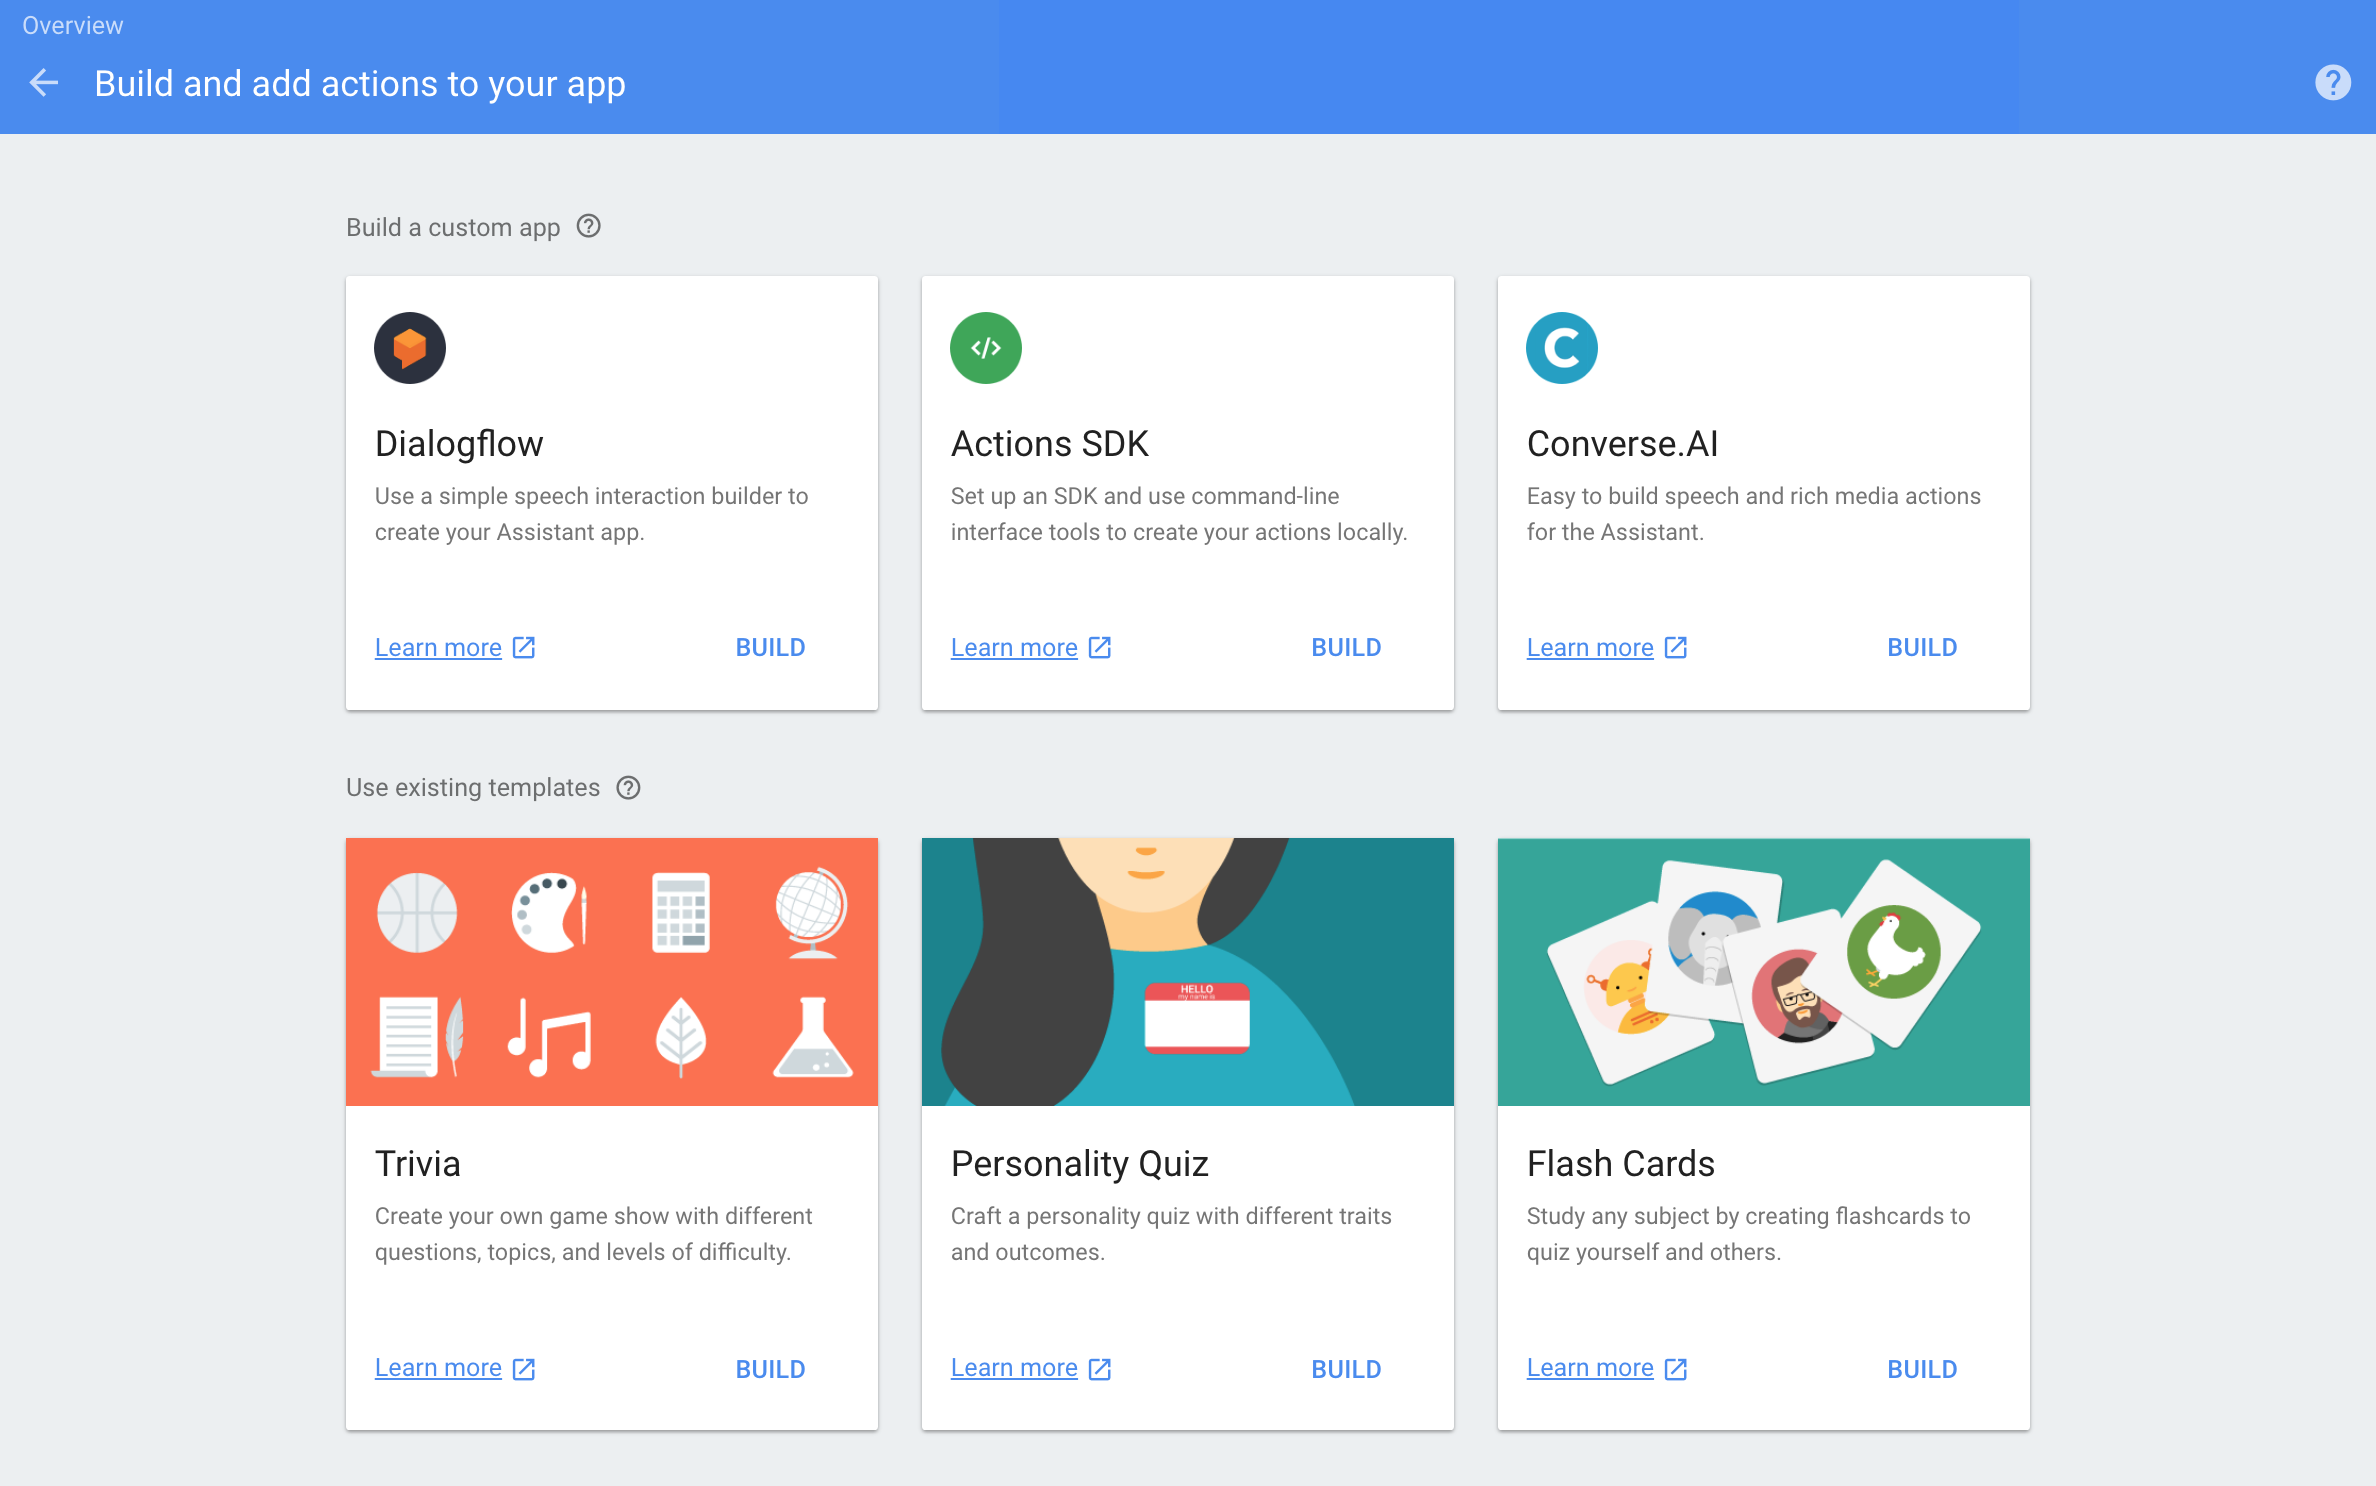
\includegraphics[width=1\linewidth]{images/script_image}
	\caption[actions_google]{Actions On Google Console}
	\label{fig:scriptimage}
\end{figure}

\end{frame}

% frame
\begin{frame}
\frametitle{Invitation/Inhibition: make your own decisions}
% Developers define what actions are possible and what are not. The scripts of artifacts suggest specific actions and discourage others. Idea: the flow won’t go on until the user has included in the answers the parameters

\begin{block}{Invitation/Inhibition} 
	\begin{quote}
		The scripts of artifacts \textbf{suggest specific actions} and \textbf{discourage others} (\cite{verbeek2011moralizing})
	\end{quote}

\begin{itemize}
	% Fullfillment}
	% to respond to the user and to complete the requested action
	\item Developers while creating the application logic (\emph{fulfillment}) \textbf{enable some actions} and \textbf{disable some others}
	% Dialogflow can extract parameters from the user input, validate the parameter and provide it to your fulfillment as a variable
	\item The conversational interaction doesn't go on if the user hasn't answered with \textbf{all the required parameters}
	%select the REQUIRED checkbox for the number parameter. This tells Dialogflow to not trigger the intent until the parameter is properly provided by the user.
\end{itemize}

\end{block}

\end{frame}

\begin{frame}
\frametitle{Invitation/Inhibition: make your own decisions}
\begin{figure}
	\centering
	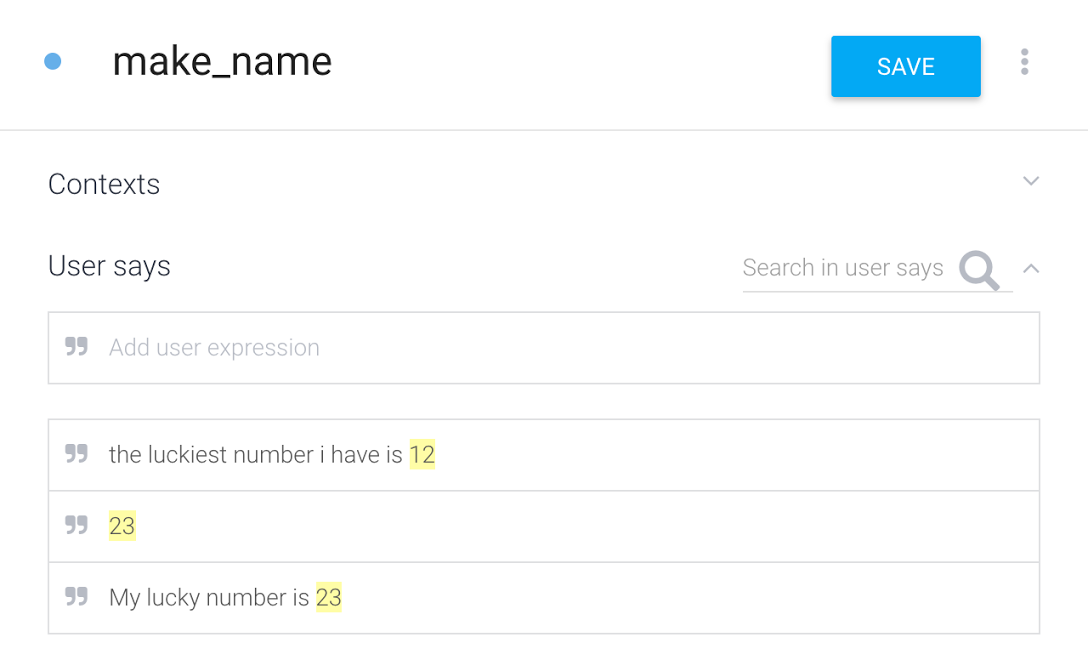
\includegraphics[width=0.75\linewidth]{images/invitation_inhibition}
	\label{fig:invitationinhibition}
\end{figure}

\begin{figure}
	\centering
	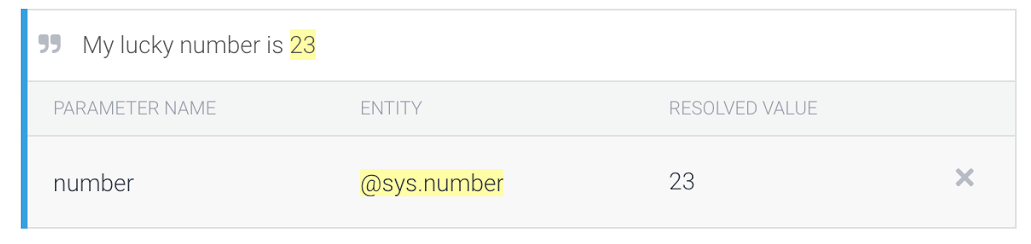
\includegraphics[width=0.7\linewidth]{images/invitation_inhibition_param}
	\label{fig:invitationinhibitionparam}
	\caption{DialogFlow interactions}
\end{figure}

\end{frame}

% frame
\begin{frame}[allowframebreaks]
\frametitle{Behaviour Steering: think freely}
%behaviour steer starts in our head and then leads to a steered action

	\begin{columns}
		\column{0.55\linewidth}
			\begin{block}{Suggestion Chips}
		 		\begin{quote}
		 			Use suggestion chips to \textbf{hint at responses} to continue or \textbf{pivot the conversation}.
		 		\end{quote}
		 			
		 		\begin{quote}
		 			If during the conversation there is a primary call for action, \textbf{consider listing that as the first suggestion chip} (\cite{googleactions})
		 		\end{quote}
	 		\end{block}
 		\bigskip
 		
 		This happens in vocal interactions but can be more easily visualized on mobile phones
	 		
		\column{0.45\linewidth}
			\centering
			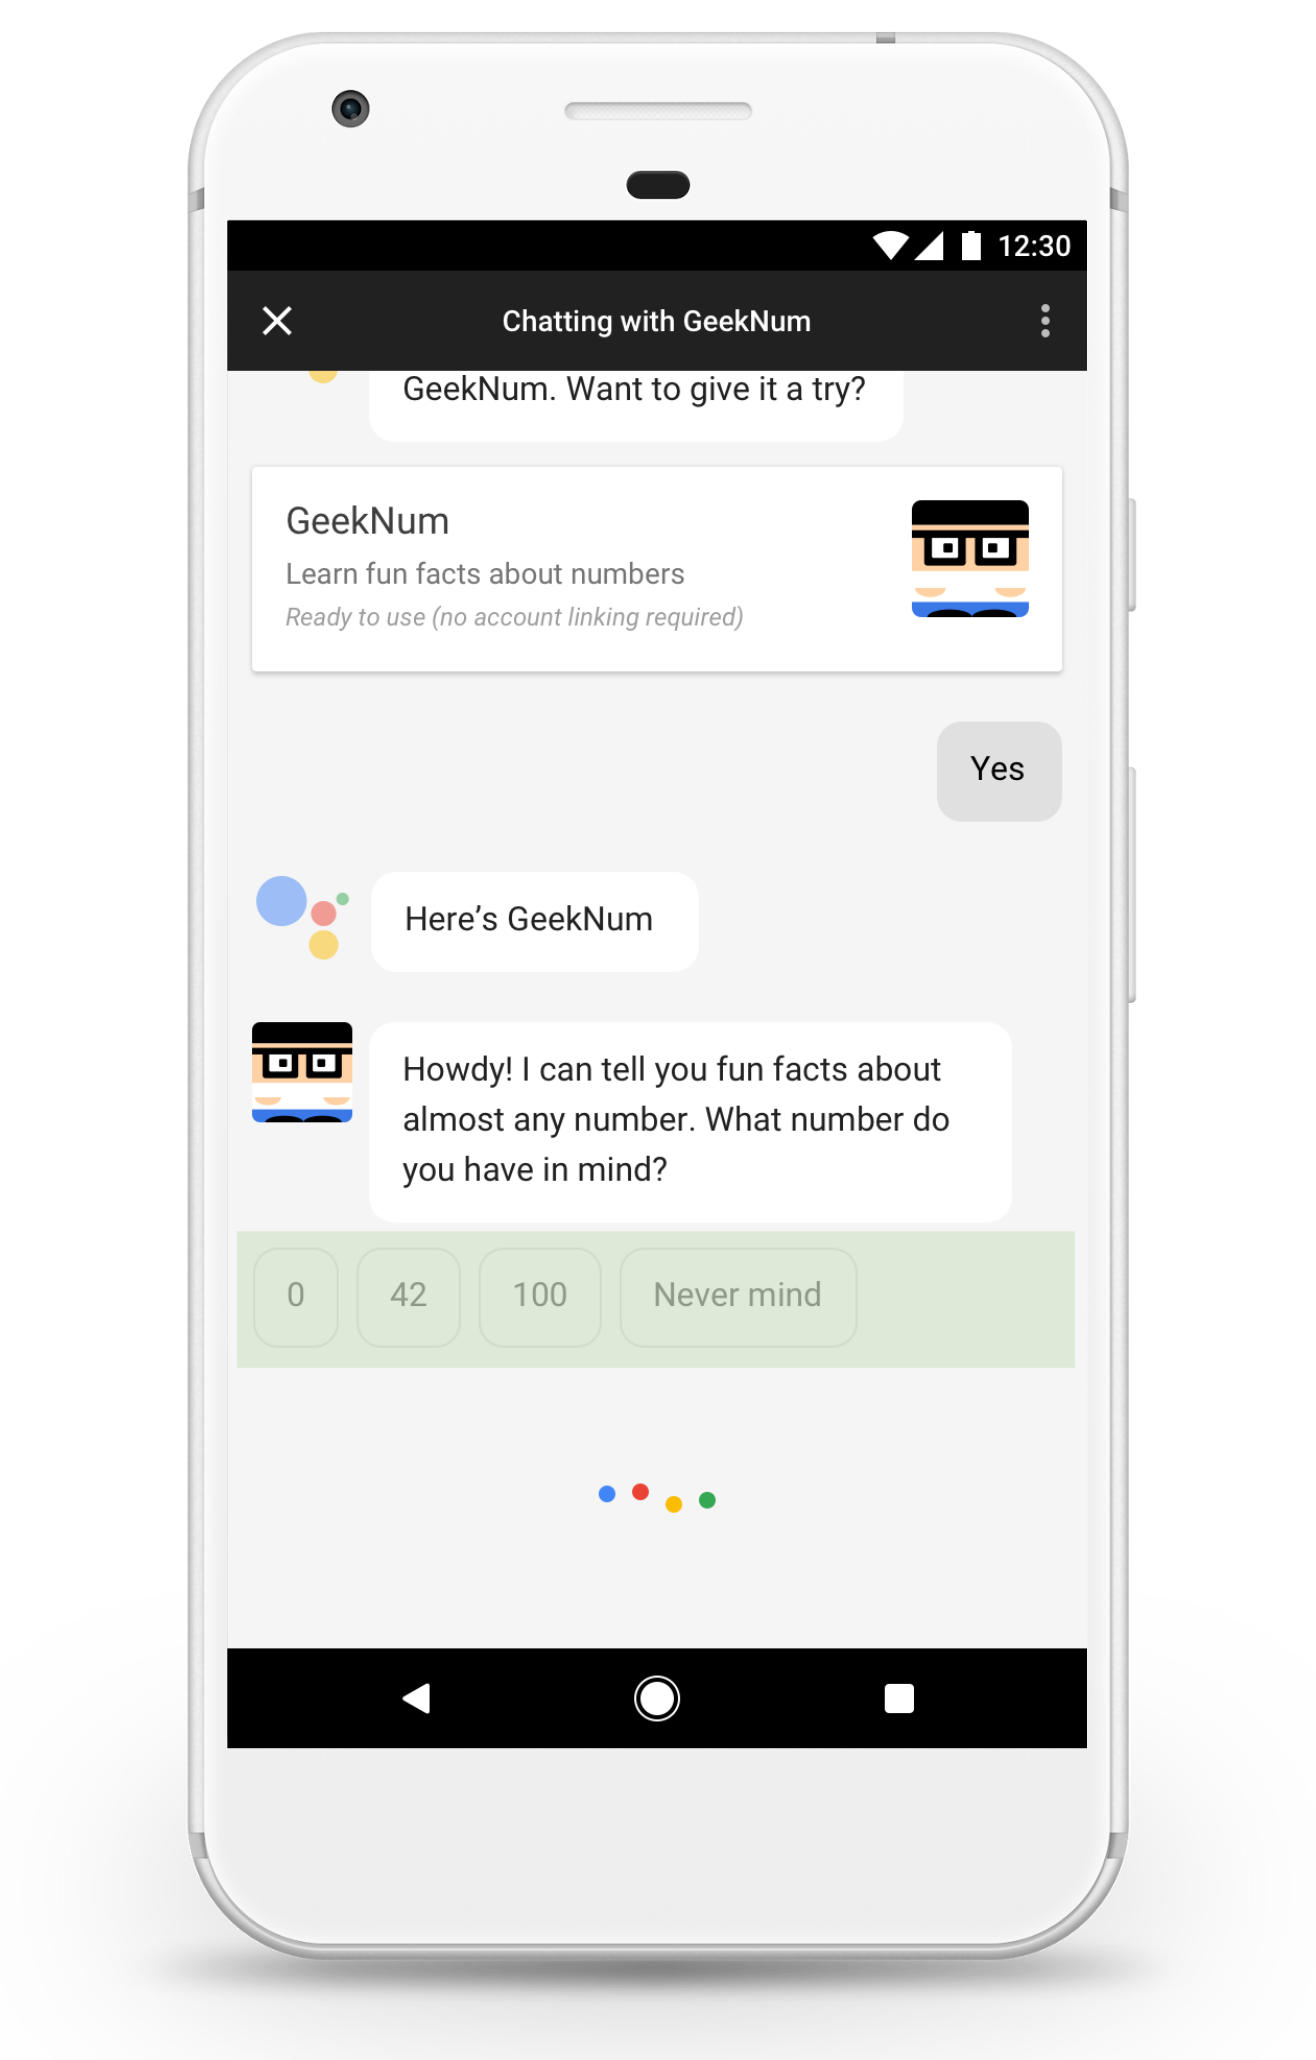
\includegraphics[width=1.0\linewidth]{images/suggestion-chip}
	\end{columns}
\framebreak

\begin{quote}
Smart objects could become \textbf{intermediaries between businesses and consumers}, using their intelligence to \textbf{persuade customers to buy products} \dots Such influence could already be \textbf{exerted at the design stage} \dots\\(\cite{brey2005freedom})
\end{quote}

\begin{block}{Advertisements}
	\begin{itemize}
		% in the middle of a normal answer to a user
		\item Google Assistant \textbf{advertised "\emph{Beauty and the Beast}"} film, but Google claimed it was not an ad (\cite{androidPolice})
		\medskip
		\item In future \textbf{Google Assistant will include ads}
			\begin{itemize}
				\item make money by \textbf{promoting e-commerce from partners} (\cite{recode})
				% Google’s vice president of ads division
				\item forecasted voice assistants ad-spend of \textbf{19 billions globally by 2022} (\cite{juniper})
			\end{itemize}
	\end{itemize}
\end{block}

\framebreak

\begin{quote}
	\textbf{Agent-based dialogue systems} can be included in IUI’s

	to monitor users and \textbf{make assumptions about their intentions and the task they are trying to perform} \\(\cite{brey2005freedom})
\end{quote}

\begin{block}{Implicit Invocation}
\begin{quote}
The Assistant opts to invoke an app because it can fulfill the user's intent, \textbf{without users calling it by name} (\cite{googleactions})
\end{quote}

\bigskip
Example: "Hey Google, book an appointment to fix my bike."
\end{block}
\end{frame}

% frame
\begin{frame}
\frametitle{Where is Technological Mediation? }
1) Google Actions Policies and terms: designed towards privacy, content, branding, … : what about technological mediation?
\end{frame}

\subsection{Ethical concerns arising from loss of freedom}
% interleave
\begin{frame}
\begin{center} 
	\usebeamerfont*{frametitle}
	\usebeamercolor[fg]{frametitle} Ethical concerns arising from loss of freedom
\end{center}
\end{frame}

% frame
\begin{frame}
	\frametitle{Technocracy}
 + we may have the opposite problem: non technical people designing actions without having enough background!!!	
\end{frame}

% frame
\begin{frame}
\frametitle{Moral Laziness}
commodification of morality
\end{frame}

% frame
\begin{frame}
	\frametitle{Moral responsibility of designers}
	What if in the future developers will shape morality??? Responsibility vacuum	
\end{frame}

% frame
\begin{frame}
\frametitle{What about behaviour change?}
what if we want to change our behaviour towards what we think is good to us and not towards what is good for the designers?
\end{frame}

\section{Possible Remedies}
% interleave
\begin{frame}
\begin{center} 
	\usebeamerfont*{frametitle}
	\usebeamercolor[fg]{frametitle} Possible Remedies
\end{center}
\end{frame}

% frame
\begin{frame}
\frametitle{Possible Remedies}
\end{frame}

% bibliography frame,see https://tex.stackexchange.com/questions/68080/beamer-bibliography-icon/68084#68084 for reference
\nocite{*}
\begin{frame}[noframenumbering,plain,allowframebreaks]{Bibliography}
\renewcommand*{\bibfont}{\small}
\printbibliography
\end{frame}

\end{document}